\subsection{Prérequis}

Pour utiliser ChromaCase, vous aurez besoin de

\begin{itemize}
	\item Un Piano avec une connectivité MIDI
	\item Un ordinateur, ou une tablette ou smartphone Android  avec une connectivité pour brancher votre piano (généralement USB)
	\item Une connexion Internet
\end{itemize}


\subsection{Fonctionnement}
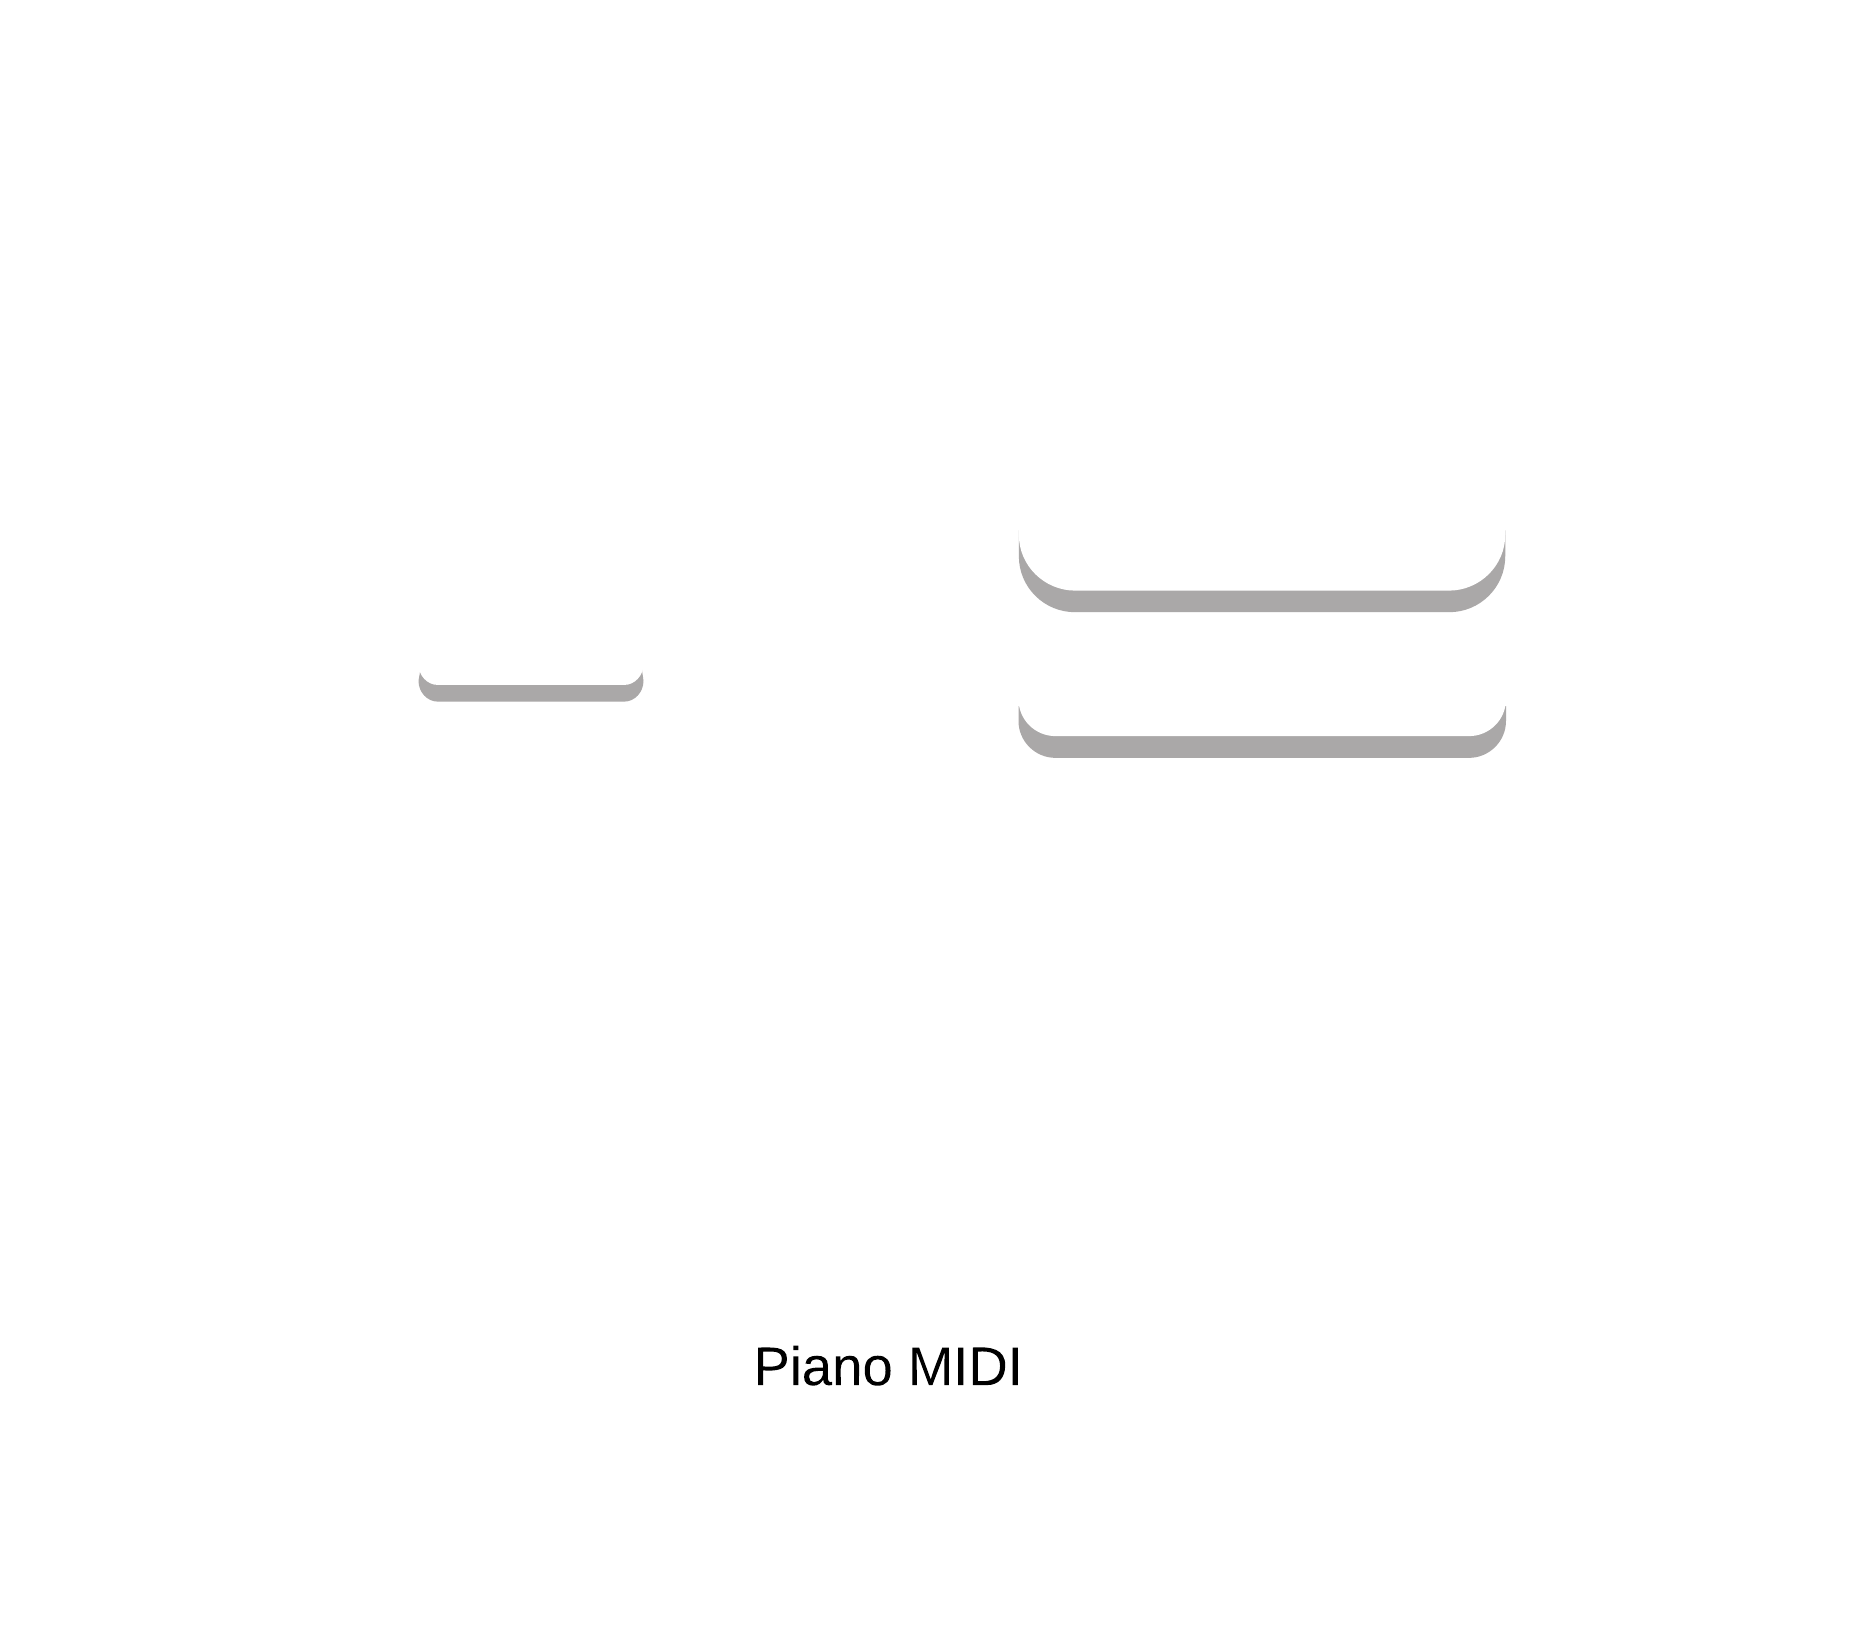
\includegraphics[width=\textwidth]{../assets/structure-front.png}

Pour fonctionner, ChromaCase récupère les notes que vous jouez sur votre Piano et les évalue en temps réel. 

\subsection{Installation \& Accès}

Avant de vous rendre sur ChromaCase, branchez votre piano à votre appareil.

\subsubsection{Web}

Vous devriez surement autoriser ChromaCase à accéder aux connexions MIDI.

Pour accéder à ChromaCase, rendez-vous sur \url{https://chroma.octohub.app/}.

Vous arriverez sur la page d'accueil, depuis laquelle vous devrez vous authentifier (ou créer un compte) pour continuer (cf. section Guide d'utilisation).

\subsubsection{Android}

Vous devriez surement autoriser ChromaCase à accéder aux connexions MIDI.

Pour accéder à l'application, téléchargez et installez le fichier nommé \texttt{android-build.apk} sur ce \href{https://github.com/Chroma-Case/Chromacase/releases}{\texttt{lien}}.

Vous arriverez sur la page d'accueil, depuis laquelle vous devrez vous authentifier (ou créer un compte) pour continuer (cf. section Guide d'utilisation).
